
The superconducting state is a phase of matter or, more precisely, 
a second-order phase transition of matter at a temperature $T_c$ that 
induces different properties. The historical property is the low resistance 
($R < 10^{-5} \Omega$) discovered by Heike Kamerlingh Onnes.


\fig{1}{part/intro/Mercury_superconducting_transition.pdf}{Mercury
superconducting
transition}

\newpage
In 1933, in Berlin, 
Walther Meissner and Robert 
Ochsenfeld showed that the magnetic 
field $B$ is “expelled” from superconductors. 
This means that when subjected to an external magnetic 
field, superconductors divert the field lines so that the 
magnetic field vanishes inside. The superconducting material 
behaves as a perfect diamagnet \cite{mangin_superconductivity_2017} p.20.

\fig{0.5}{part/intro/EfektMeisnera.pdf}{Diagram of the  Meissner-Ochsenfeld effect. 
Magnetic field lines $\mathbf{B}$, represented as arrows,
 are excluded from a superconductor when it is below its critical temperature $T_c$ \cite{mangin_superconductivity_2017}.}



\mydef{Cooper pairs}{
Is a pair of two fermions with a opposite spin and momentum
\begin{center}
    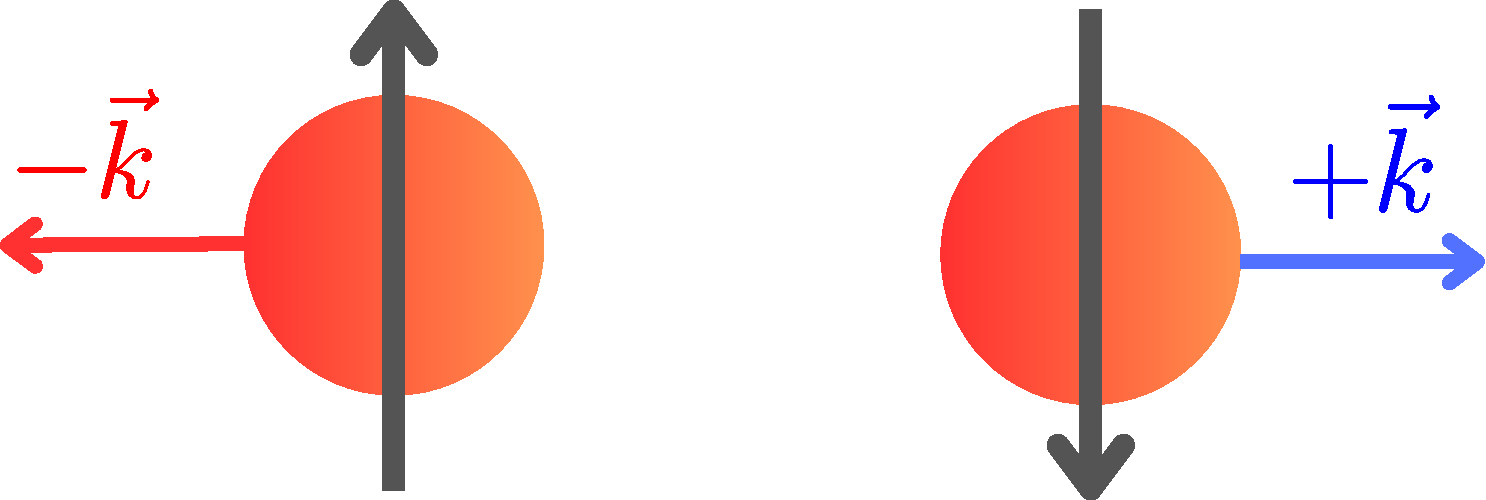
\includegraphics[width=0.6\linewidth]{part/intro/Cooper_pairs.pdf}
\end{center}

}


\myth{Type of particule}{

The Cooper pairs are bosons

}

\begin{proof}
    The spin of the Cooper in equal to zero, by consequese 
    of the statistical theorem the Cooper pairs are bosons.
\end{proof}



The microscopic wave function of the system of Cooper pairs 

\begin{equation}
    \psi (\vec{r}_1, \vec{r}_2, \cdots, \vec{r}_N, t )
    = \varphi(\vec{r}_1,t)\varphi(\vec{r}_2,t)\cdots\varphi(\vec{r}_N,t)
\end{equation}

and $\varphi(\vec{r}_i,t)$ : describes the wavefunction of 
a single Cooper pair at the time $t$ and the position $\vec{r}_i$


Is mean Field approach ! (or the wave function
is a seperable state in quantum information)


\mydef{Mean Field Theory}{

The main idea of MFT is to replace all interactions to any one body with an average or effective interaction, sometimes called a molecular field.[1] This reduces any 
many-body problem into an effective one-body problem.
}





\newpage

\subsection{Current density and the LONDON equation}
Hypothesis :

COOPER pairs will be considered in this chapter as ``particles'' of mass $m_p$ and charge $q_p$ double those of an electron, and whose density $n_p$ is half that of superconducting electrons:
\[
m_p = 2m \, ; \quad q_p = -2e \, ; \quad n_p = \frac{n_s}{2}
\]


And why now experiementaly at
the temperature $T_c$ the Cooper pairs condensate 
we can write the macroscopic wave function of the system of 
many Cooper pairs in polar representation
\begin{equation*}
    \Psi (\vec{r}, t) = \sqrt{n_s(\vec{r}, t)} e^{i \theta (\vec{r}, t)}
\end{equation*}


where :
\begin{itemize}
    \item $n_s$ : density of charge carrier (Cooper pair)
    \item $\theta$ : superconducting phase
\end{itemize}

\myprop{Hamiltionan of charge particles}{
    The Hamiltonian for a system of 
    charged particles in an electromagnetic 
    field is given by:

\begin{equation}
    \hat{H} = \sum_{i} \left( \frac{1}{2m_i} \left( \hat{\mathbf{p}}_i - q_i \mathbf{A}(\hat{\mathbf{r}}_i) \right)^2 + q_i \phi(\hat{\mathbf{r}}_i) \right) + \frac{1}{2} \sum_{i \neq j} \frac{q_i q_j}{4\pi \epsilon_0 |\hat{\mathbf{r}}_i - \hat{\mathbf{r}}_j|}
\end{equation}


\begin{itemize}
    \item $\hat{H}$ is the Hamiltonian operator for the system.
    \item $m_i$ is the mass of the $i$-th particle.
    \item $\hat{\mathbf{p}}_i$ is the momentum operator of the $i$-th particle.
    \item $q_i$ is the charge of the $i$-th particle.
    \item $\mathbf{A}(\hat{\mathbf{r}}_i)$ is the vector potential of the electromagnetic field at the position $\hat{\mathbf{r}}_i$ of the $i$-th particle.
    \item $\phi(\hat{\mathbf{r}}_i)$ is the scalar potential of the electromagnetic field at the position $\hat{\mathbf{r}}_i$ of the $i$-th particle.
    \item $\epsilon_0$ is the permittivity of free space and $|\hat{\mathbf{r}}_i - \hat{\mathbf{r}}_j|$ is the distance between the $i$-th and $j$-th particles.
\end{itemize}
}

\begin{proof}
    cf book of Electrodynamics
\end{proof}

\myth{London equations}{

The London equations describe the electromagnetic properties of superconductors. One of the London equations can be written as:

\begin{equation}
\nabla \times \mathbf{J} = -\frac{n_s e^2}{m} \mathbf{B}
\end{equation}

where:
\begin{itemize}
    \item $\mathbf{J}$ is the superconducting current density,
    \item $n_s$ is the density of superconducting electrons,
    \item $e$ is the charge of an electron,
    \item $m$ is the mass of an electron,
    \item $\mathbf{B}$ is the magnetic field.
\end{itemize}

}


\begin{proof}
    
\end{proof}


\textbf{Rq:} A major triumph o
f the equations is their 
ability to explain the Meissner effect,
wherein a material exponentially expels 
all internal magnetic fields as it 
crosses the superconducting threshold.